% INVERSE PROBLEMS
\textit{Inversion} is the inference of model parameters from noisy and limited data and is often formulated as statistical estimation.
This formulation encompasses a wide range of problems.
% CLASSICAL INVERSION
\textit{Parameter estimation} \cite{Bayesian:Hadidi2008,Bayesian:Beck2010} aims at inferring unknown parameters \(\bm{x} \in \mathds{R}^m\) of a physical forward model \(\mathcal{M}\).
This model predicts the outcome \(\mathcal{M}(\bm{x},\bm{d}_i)\) of \(i=1,\ldots,n\) experiments under known experimental conditions \(\bm{d}_i\).
% RESIDUAL MODELS
The discrepancy between predictions and real data \(\bm{y}_i\) is accounted for by a statistical model \(\bm{y}_i = \mathcal{M}(\bm{x},\bm{d}_i) + \bm{\varepsilon}_i\).
Here the residuals \(\bm{\varepsilon}_i \sim f_{\bm{E}_i}(\bm{\varepsilon}_i)\) capture measurement errors, numerical approximations and model inadequacies.
A widespread probabilistic formulation rests on independent Gaussian distributions \(f_{\bm{E}_i}(\bm{\varepsilon}_i) = \mathcal{N}(\bm{\varepsilon}_i \cond \bm{0},\bm{\Sigma}_i)\) with covariance matrices \(\bm{\Sigma}_i\).
% BAYESIAN UPDATING
In Bayesian inversion the prior distribution \(\pi(\bm{x})\) quantifies the epistemic parameter uncertainty of the quantities of interest (QoI) \(\bm{x}\) before the data are analyzed.
With the likelihood function \(\mathcal{L} (\bm{x}) = \prod_{i=1}^n f_{\bm{E}_i} (\bm{y}_i-\mathcal{M}(\bm{x},\bm{d}_i))\)
the posterior probability density follows through Bayes' law \(\pi(\bm{x} \cond \tuple{\bm{y}_i}) \propto \mathcal{L}(\bm{x}) \, \pi(\bm{x})\).
Here the data from all experiments are denoted as \(\tuple{\bm{y}_i} = (\bm{y}_1,\ldots,\bm{y}_n)\).
The posterior represents the knowledge about the unknown parameter vector after conditioning on the data.
% MARKOV CHAIN MONTE CARLO
Apart from exceptional cases the posterior has no analytically closed form, thus more often than not the challenge lies in sampling the posterior by means of MCMC \cite{MCMC:Robert2004,MCMC:Brooks2011}.
\par % MULTILEVEL INVERSION
Another type of inverse problem arises when variations in the data \(\bm{y}_i\) are not only attributed to different conditions \(\bm{d}_i\) and random residuals \(\bm{\varepsilon}_i\),
but also as a consequence of naturally varying forward model inputs \(\bm{x}_i\).
Throughout the experiments \(i=1,\ldots,n\) those inputs take on unobservable realizations of conditionally independent random variables
\((\bm{x}_i \cond \bm{\theta}_{\bm{X}}) \sim f_{\bm{X} \cond \bm{\Theta}_{\bm{X}}} (\bm{x}_i \cond \bm{\theta}_{\bm{X}})\).
This conditional distribution represents aleatory variability.
Data are then represented as \(\bm{y}_i = \mathcal{M}(\bm{x}_i,\bm{d}_i) + \bm{\varepsilon}_i\).
Prior to data analysis the distribution \(\pi(\bm{\theta}_{\bm{X}})\) encodes the epistemic uncertainty of the hyperparameters \(\bm{\theta}_{\bm{X}}\).
% HIERARCHICAL MODEL
The described experimental situation is summarized as the hierarchical model
\begin{subequations} \label{eq:Multilevel:Model}
  \begin{align}
    (\bm{y}_i \cond \bm{x}_i) &\sim f_{\bm{E}_i} (\bm{y}_i-\mathcal{M}(\bm{x}_i,\bm{d}_i)), \\
    (\bm{x}_i \cond \bm{\theta}_{\bm{X}}) &\sim f_{\bm{X} \cond \bm{\Theta}_{\bm{X}}} (\bm{x}_i \cond \bm{\theta}_{\bm{X}}), \\
    \bm{\theta}_{\bm{X}} &\sim \pi (\bm{\theta}_{\bm{X}}).
  \end{align}
\end{subequations}
In \cref{fig:DAG} this model is visualized as a directed acyclic graph (DAG).
Here nodes represent known or unknown quantities while directed edges represent probabilistic or deterministic relations.
% FIGURE: DAG
\begin{figure}[ht]
  \centering
  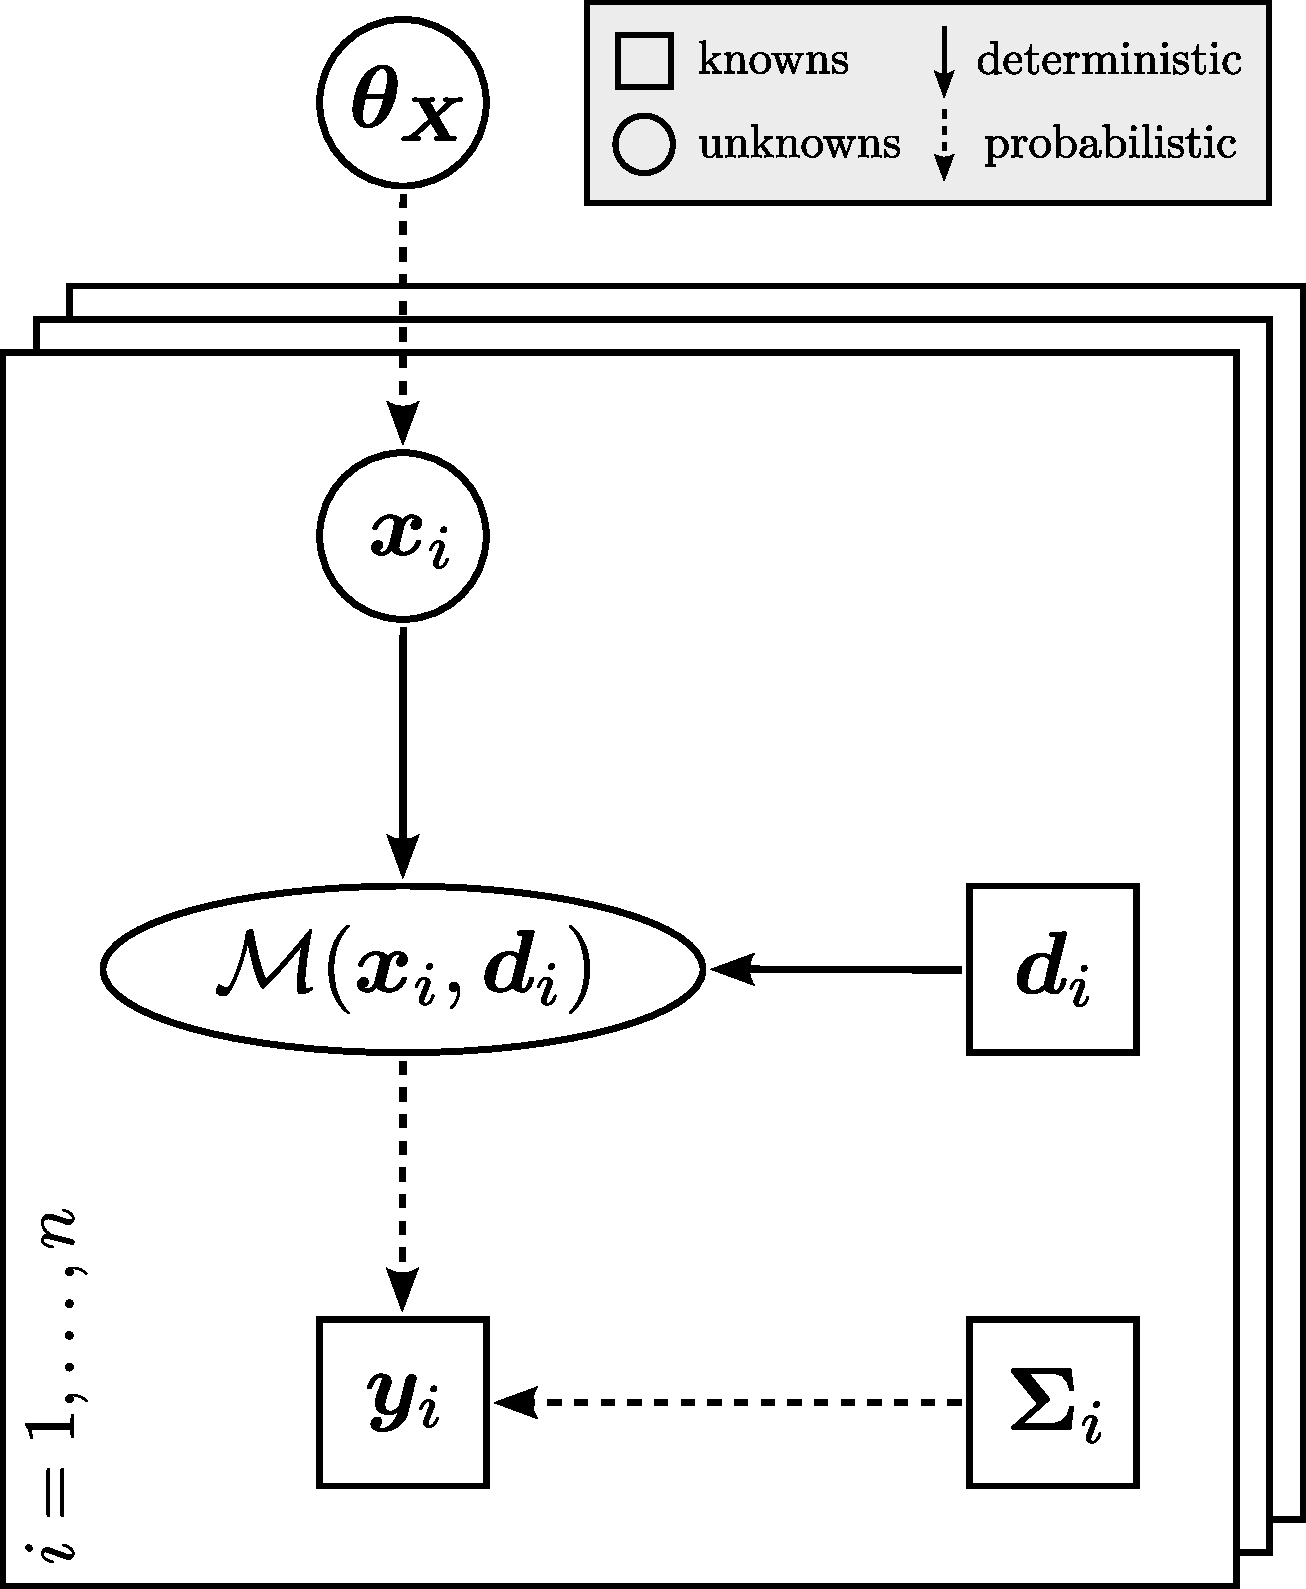
\includegraphics[width=\JRUESdagWidth]{fig_JRUES_ProbInv}
  \caption[DAG of the multilevel model]{DAG of the multilevel model.}
  \label{fig:DAG}
\end{figure}
\par % MARGINALIZED LIKELIHOOD
\textit{Probabilistic inversion} \cite{Multilevel:Rocquigny2009,Multilevel:Celeux2010,Multilevel:Barbillon2011} is the problem of estimating the unknown hyperparameters \(\bm{\theta}_{\bm{X}}\) that are the QoI.
A likelihood for this class of problems can be obtained by the marginalization
\(\mathcal{L} (\bm{\theta}_{\bm{X}}) = \prod_{i=1}^n \int f_{\bm{E}_i} (\bm{y}_i-\mathcal{M}(\bm{x}_i,\bm{d}_i)) \, f_{\bm{X} \cond \bm{\Theta}_{\bm{X}}} (\bm{x}_i \cond \bm{\theta}_{\bm{X}}) \, \mathrm{d} \bm{x}_i\).
The posterior \(\pi(\bm{\theta}_{\bm{X}} \cond \tuple{\bm{y}_i}) \propto \mathcal{L}(\bm{\theta}_{\bm{X}}) \, \pi(\bm{\theta}_{\bm{X}})\) results from Bayes' theorem.
% PRACTICALLY
In practice the integrated likelihood can be computed through stochastic integration \cite{Nagel:IPW2013:Proc} or Laplace's method \cite{Multilevel:Ballesteros2014:Proc}.
% JOINT POSTERIOR
\textit{Multilevel inversion} \cite{Nagel:JAIS2015,Nagel:PEM2016} is the joint estimation of all unknowns \((\tuple{\bm{x}_i},\bm{\theta}_{\bm{X}})\) by conditioning on all knowns \(\tuple{\bm{y}_i}\).
The corresponding joint posterior distribution is given as
\begin{equation} \label{eq:Multilevel:Posterior}
  \pi(\tuple{\bm{x}_i},\bm{\theta}_{\bm{X}} \cond \tuple{\bm{y}_i}) \propto
  \left( \prod\limits_{i=1}^n f_{\bm{E}_i} (\bm{y}_i-\mathcal{M}(\bm{x}_i,\bm{d}_i)) \right)
  \left( \prod\limits_{i=1}^n f_{\bm{X} \cond \bm{\Theta}_{\bm{X}}}(\bm{x}_i \cond \bm{\theta}_{\bm{X}}) \right) \pi(\bm{\theta}_{\bm{X}}).
\end{equation}
% BORRWOING STRENGTH
On the one side, the posterior \cref{eq:Multilevel:Posterior} offers the possibility to pool information.
Individual realizations \(\bm{x}_i\) can be optimally inferred.
This is known as \textit{optimal combination of information} or simply as \textit{borrowing strength} \cite{Multilevel:Draper1992}.
In the subsequent section this possibility is investigated.
% MCMC
On the downside, the high-dimensionality of the parameter space is a serious challenge that may necessitate advanced MCMC sampling schemes.
% DIMENSIONALITY
The number of parameters in the vector determines the dimensionality of the parameter space.
Let \(l\) and \(m\) denote the dimensions of the spaces of the unknowns \(\bm{\theta}_{\bm{X}}\) and \(\bm{x}_i\), respectively.
Then the posterior in \cref{eq:Multilevel:Posterior} involves a \((l + m \cdot n)\)-dimensional parameter space, i.e.\ the dimension grows linearly with the sample size \(n\).
Unfortunately this means that the computational cost increases with the number of experiments conducted.
In order to ameliorate this situation, HMC is later proposed as an efficient means to explore joint posteriors of the form \cref{eq:Multilevel:Posterior}.